\subsection{Shorter Not Equal Faster}

\begin{figure}
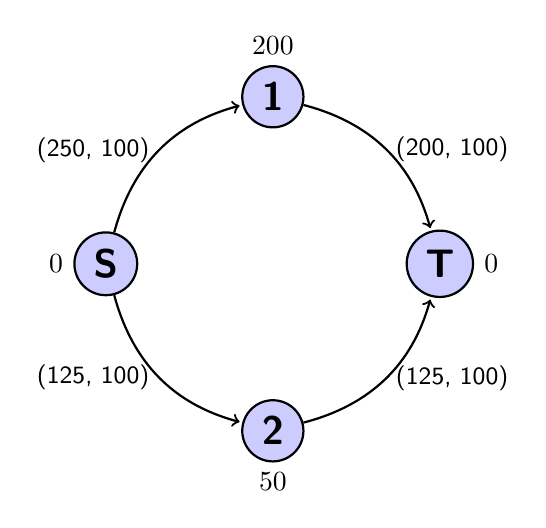
\begin{tikzpicture}[->,->,shorten >=1pt,auto,node distance=3cm,
  thick,main node/.style={circle,fill=blue!20,draw,font=\sffamily\Large\bfseries}]
%1
  \node[main node] (1) {1};
  \node[above] at (1.north) {200};
%2 
 \node[main node] (2) [below left of=1] {S};
  \node[left] at (2.west) {0};
%3 
 \node[main node] (3) [below right of=2] {2};
  \node[below] at (3.south) {50};
%4 
 \node[main node] (4) [below right of=1] {T};
  \node[right] at (4.east) {0};
%paths
  \path[every node/.style={font=\sffamily\small}]
    (1)
      edge [bend left] node[right] {(200, 100)} (4)
    (2) edge [bend right] node[left] {(125, 100)} (3)
          edge [bend left] node[left] {(250, 100)} (1)
    (3) edge [bend right] node[right] {(125, 100)} (4)
    (4) ;
\end{tikzpicture}

\label{figure:simpleroad-network}
\caption{A simple road-network with starting point s and end point t}
\end{figure}
A shorter path does not necessarily mean a faster path for electrical vehicles. 
This is partly due to the fact that an electrical vehicles uses exponentially more energy 
as its speed increases but also due to the fact that charge times on charge stations
varies a lot. Driving a longer path with a fast charge station on can therefore turn out to
be a faster choice than driving a shorter path with a slow charge station on. This is illustrated 
in Figure~\Cref{fig:simpleroad-network}. In the example we assume our car has a battery capacity of 100 kWh and a energy-usages of
0,4 kWh/km. Path 1 consist of two edges with distance = 250 km and speed limit = 100 km/t
and a charge station with a charge speed of 200 kWh/t. Path 2 consist of two edges with
distance 200 km and speed limit 100 km/t and a charge station with a charge speed of 30 kWh/t.
The total time of each path:
				
\textbf{Path 1:} \text{route time} = ((250km + 250km) / 100km/h) + (100kWh / 200kWh/h) = 5,5h
				
\textbf{Path 2:} \text{route time} = ((200 km + 200 km) / 100 km/h) + (60 kWh / 30 kWh/h) = 6 h